Algoritmi strojnog učenja ovise o dostupnim podacima.
Ne samo o broju već i kvaliteti.
Metode nadziranog učenja (\emph{eng. Supervised learning}) uz same podatke moraju na raspolaganju imati i oznaku (\emph{eng. Label}) koja definira točno što je svaki podatak prema čemu se uspoređuju i sami izlazi modela.
U puno slučajeva oznake se unose ručno što je dugotrajan i težak proces podložan greškama.
Nenadzirano učenje (\emph{eng. Unsupervised learning}) je privlačno zbog mogućnosti pronalaska i učenja distribucije danih podataka bez potrebe oznaka (\cite{ev_var_ae}).

Generativni modeli osim rješavanja danog problema, tijekom tog procesa \emph{uče} o samim podacima.
Pretpostavka je da podaci nisu u potpunosti nasumični već da dolaze u određenoj distribuciji.
Model se toj distribuciji prilagođava te ima sposobnost generiranja sintetičkih podataka koji joj odgovaraju.
Ovo poglavlje i rad fokusirati će se na model \texttt{Varijacijskog autoenkodera} (\emph{eng. Variational AutoEncoder}). \\
U nastavku se nalazi detaljnije opisan rad modela, implementacija, rezultati implementacije i poteškoće koje se javljaju.

\subsection{Varijacijski autoenkoder}
Varijacijski autoenkoder je generativni model učen nenadzirano.
Uz skup podataka $\boldsymbol{X} \in \mathbb{R}^{m \times n}$ s $m$ vektora podataka skupa $\mathbb{R}^{n}$ pretpostavlja se da podaci odgovaraju distribuciji $p(\boldsymbol{x}|\boldsymbol{z})$.
Parametar $\boldsymbol{z}$ odgovara uzorcima distribucije $p(\boldsymbol{z})$ iz \emph{latentnog prostora} (\emph{eng. latent space}) (\cite{ev_var_ae}).
Latentni prostor je niže dimenzije od $\boldsymbol{x}$.
Konačna distribucija $p(\boldsymbol{x})$ računa se kao
$$p(x) = \int p(\boldsymbol{x} | \boldsymbol{z})p(\boldsymbol{z})d\boldsymbol{z}$$
Iz danih podataka i uzorkovanja istih moguće je izračunati približne parametre distribucije što je i sama zadaća varijacijskog autoenkodera.
Nenadzirano učenje vrši se direktnom usporedbom ulaza i dobivenog konačnog izlaza.
Želja je što vjernije reproducirati ulazne vektore.

\subsubsection{Arhitektura}

\begin{figure}[H]
	\centering
	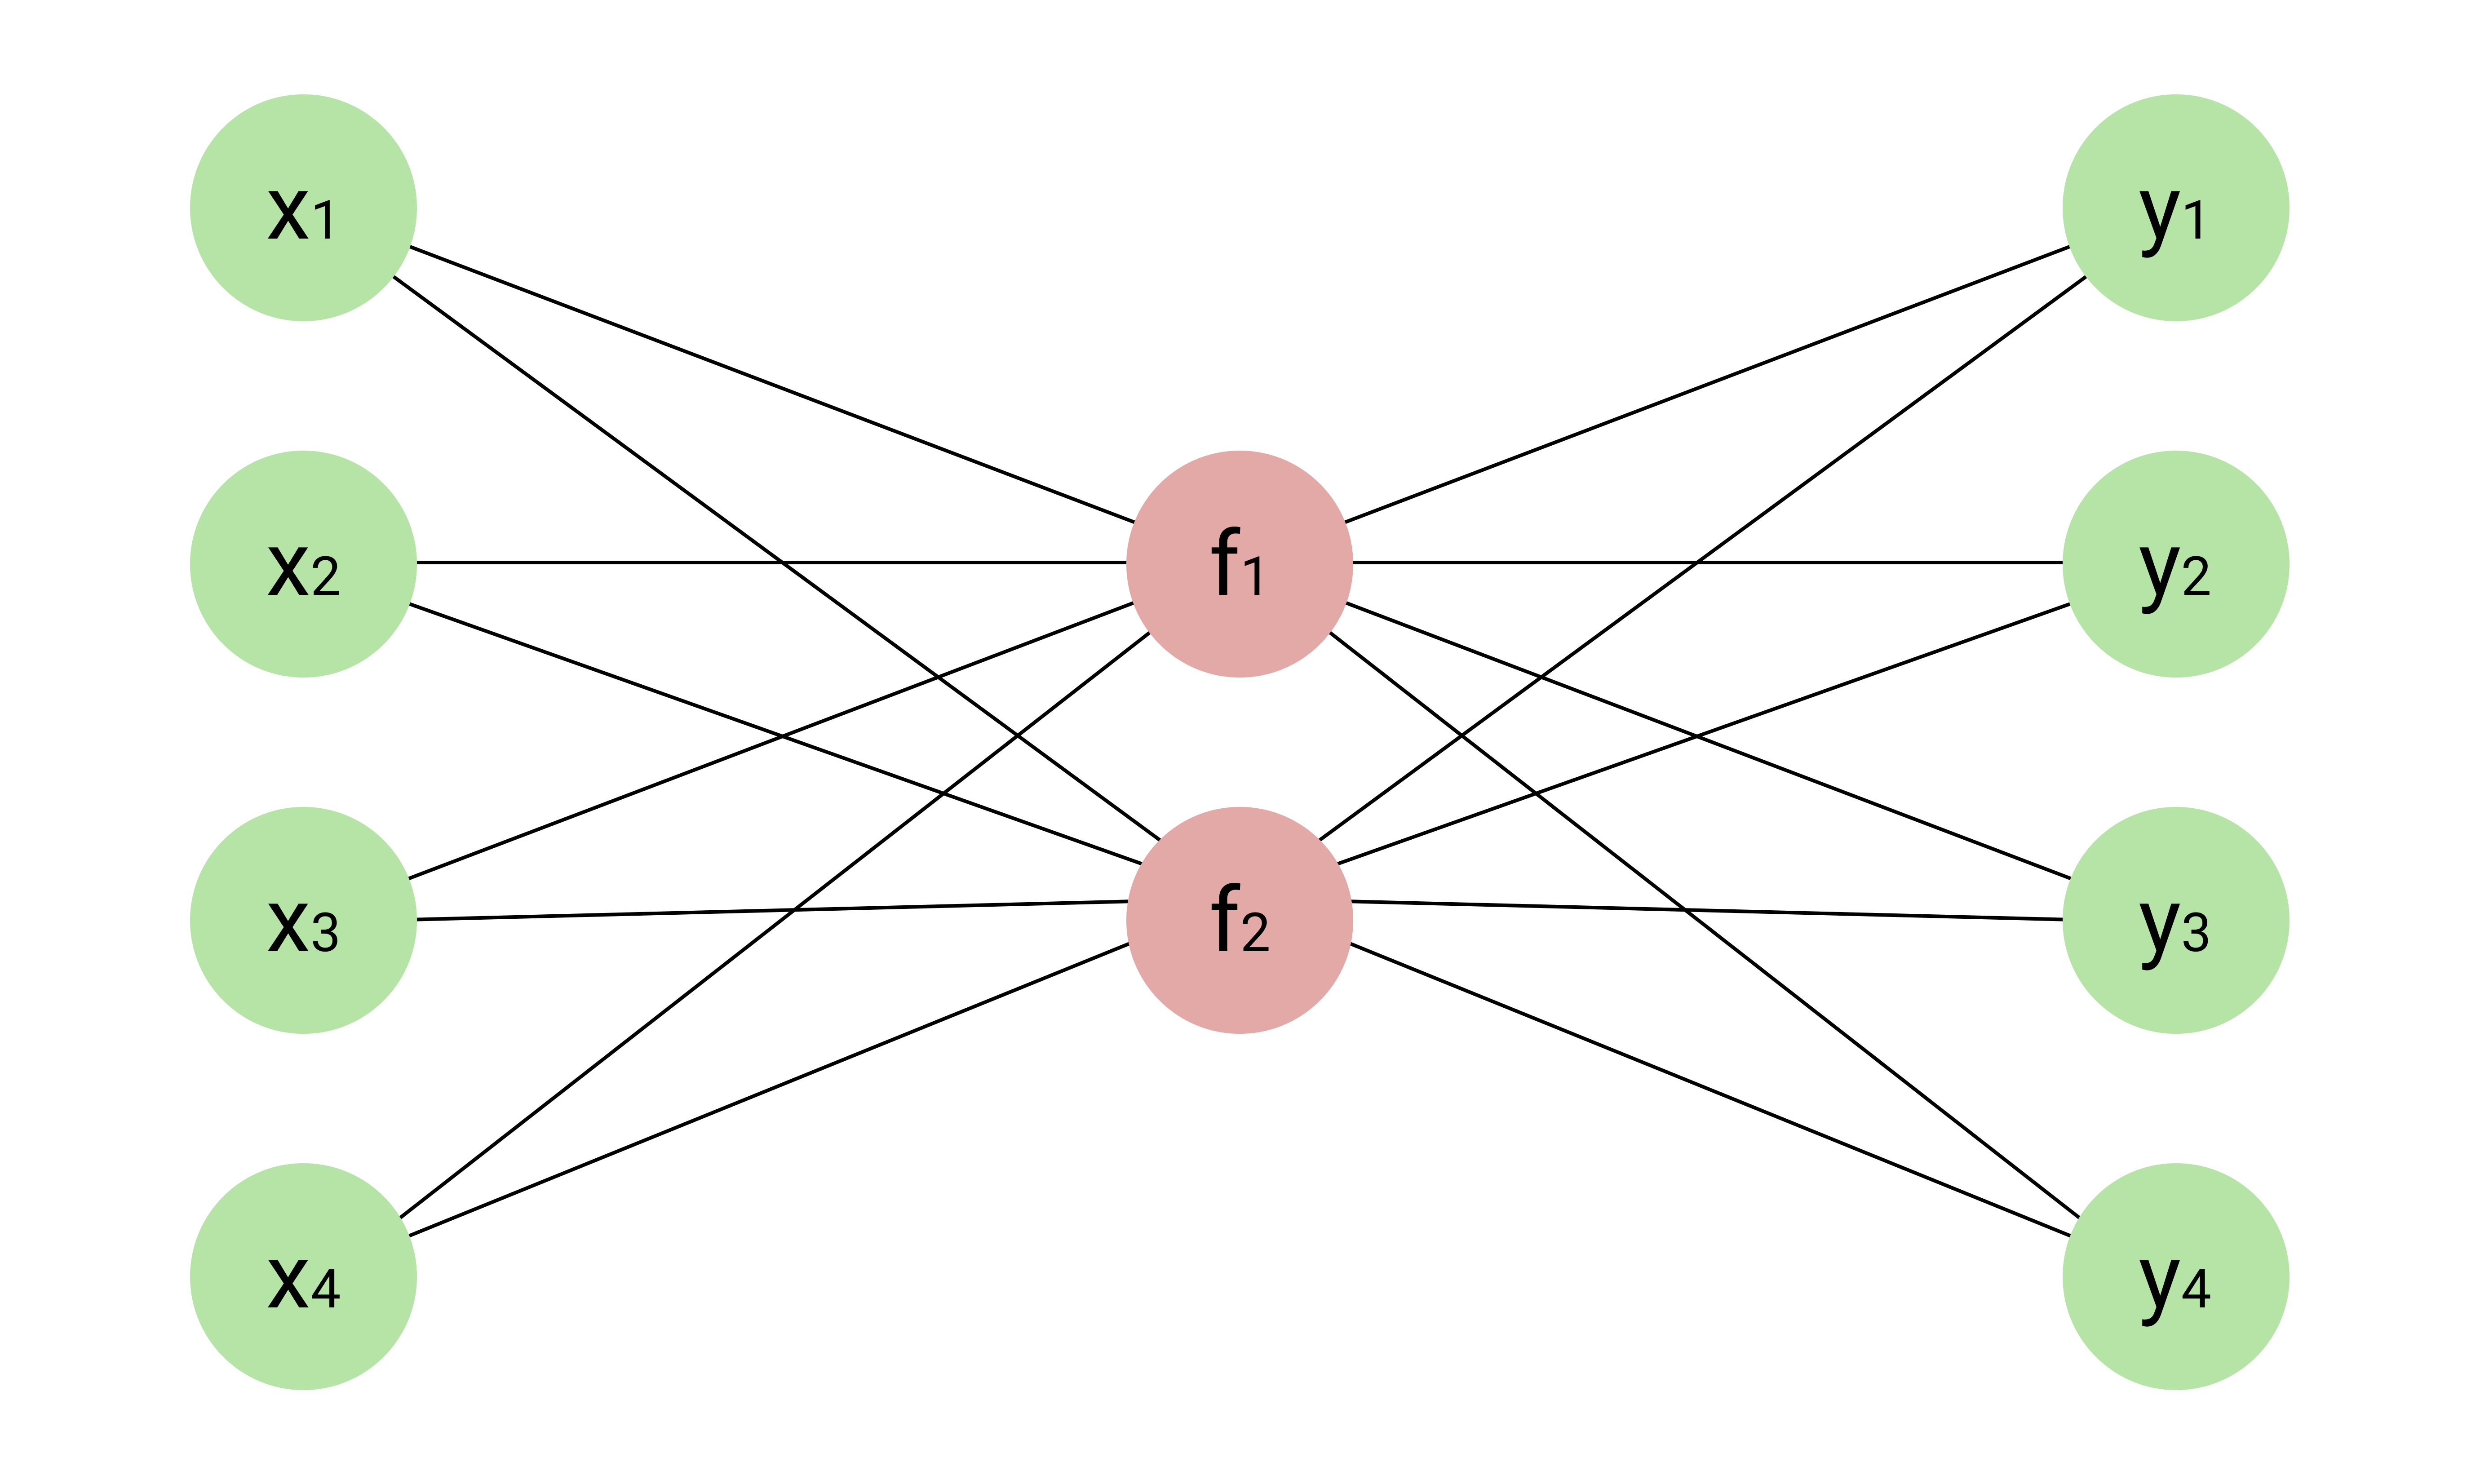
\includegraphics[width=0.8\linewidth]{Illustrations/encoder_example.png}
	\caption{Jednostavan primjer autoenkodera}
	\label{fig:autoencoder_example}
\end{figure}

Pojednostavljena arhitektura autoenkodera vidljiva je na slici \ref{fig:autoencoder_example}.
Izlazni vektor $[y_1 \cdots y_n]$ treba biti što sličniji ulaznom $[x_1 \cdots x_n]$ bez direktnog kopiranja već uz distribuciju prametriziranu s $[f_1 \cdots f_n]$.

\textbf{Enkoder} je prvi dio modela, između ulaza i skrivenog sloja iz ulaza stvara bitne značajke koje mu odgovaraju.
\textbf{Dekoder} iz značajki nastalih od enkodera čini transformaciju do izlaza. \\
Ključ je u srednjem, skrivenom sloju.
Prisiljava model na učenje samo bitnih značajki, redukciju dimenzionalnosti i izbjegavanje direktnog kopiranja.
Konačno, dekoder se može koristiti kao zasebni, generativni model koji iz danih parametara $[f_1 \cdots f_n]$ može generirati izlaz.
\subsection{Kartezijsko genetsko programiranje za generiranje podataka, CGPAE}
Genetsko programiranje je rijetko korišten alat za probleme koji se rješavaju nenadziranim učenjem.
Po mojim znanjima, ne postoji rad koji koristi Kartezijsko genetsko programiranje za izvedbu autoenkodera.
\cite{why_ae_diff} koristi jednostavan linearni genetski program s više ulaza i izlaza (LGP) umjesto CGP-a.
Smatram da je CGP fleksibilniji i ima veće računalne mogućnosti te pruža veći potencijal za bolje rezultate.
Željeni rezultat je osim uspješnog modela, model koji nosi prednosti genetskog programiranja kao što je čitljivost funkcija koje izvode enkoder i dekoder.

U prijašnjim poglavljima CGP je pokazao dobre rezultate u konvoluciji slike.
Dobre performanse u simboličkoj regresiji su također poznate.
S tim na umu, autoenkoder se čini kao moguć zadatak za riješiti.

\begin{figure}[H]
	\centering
	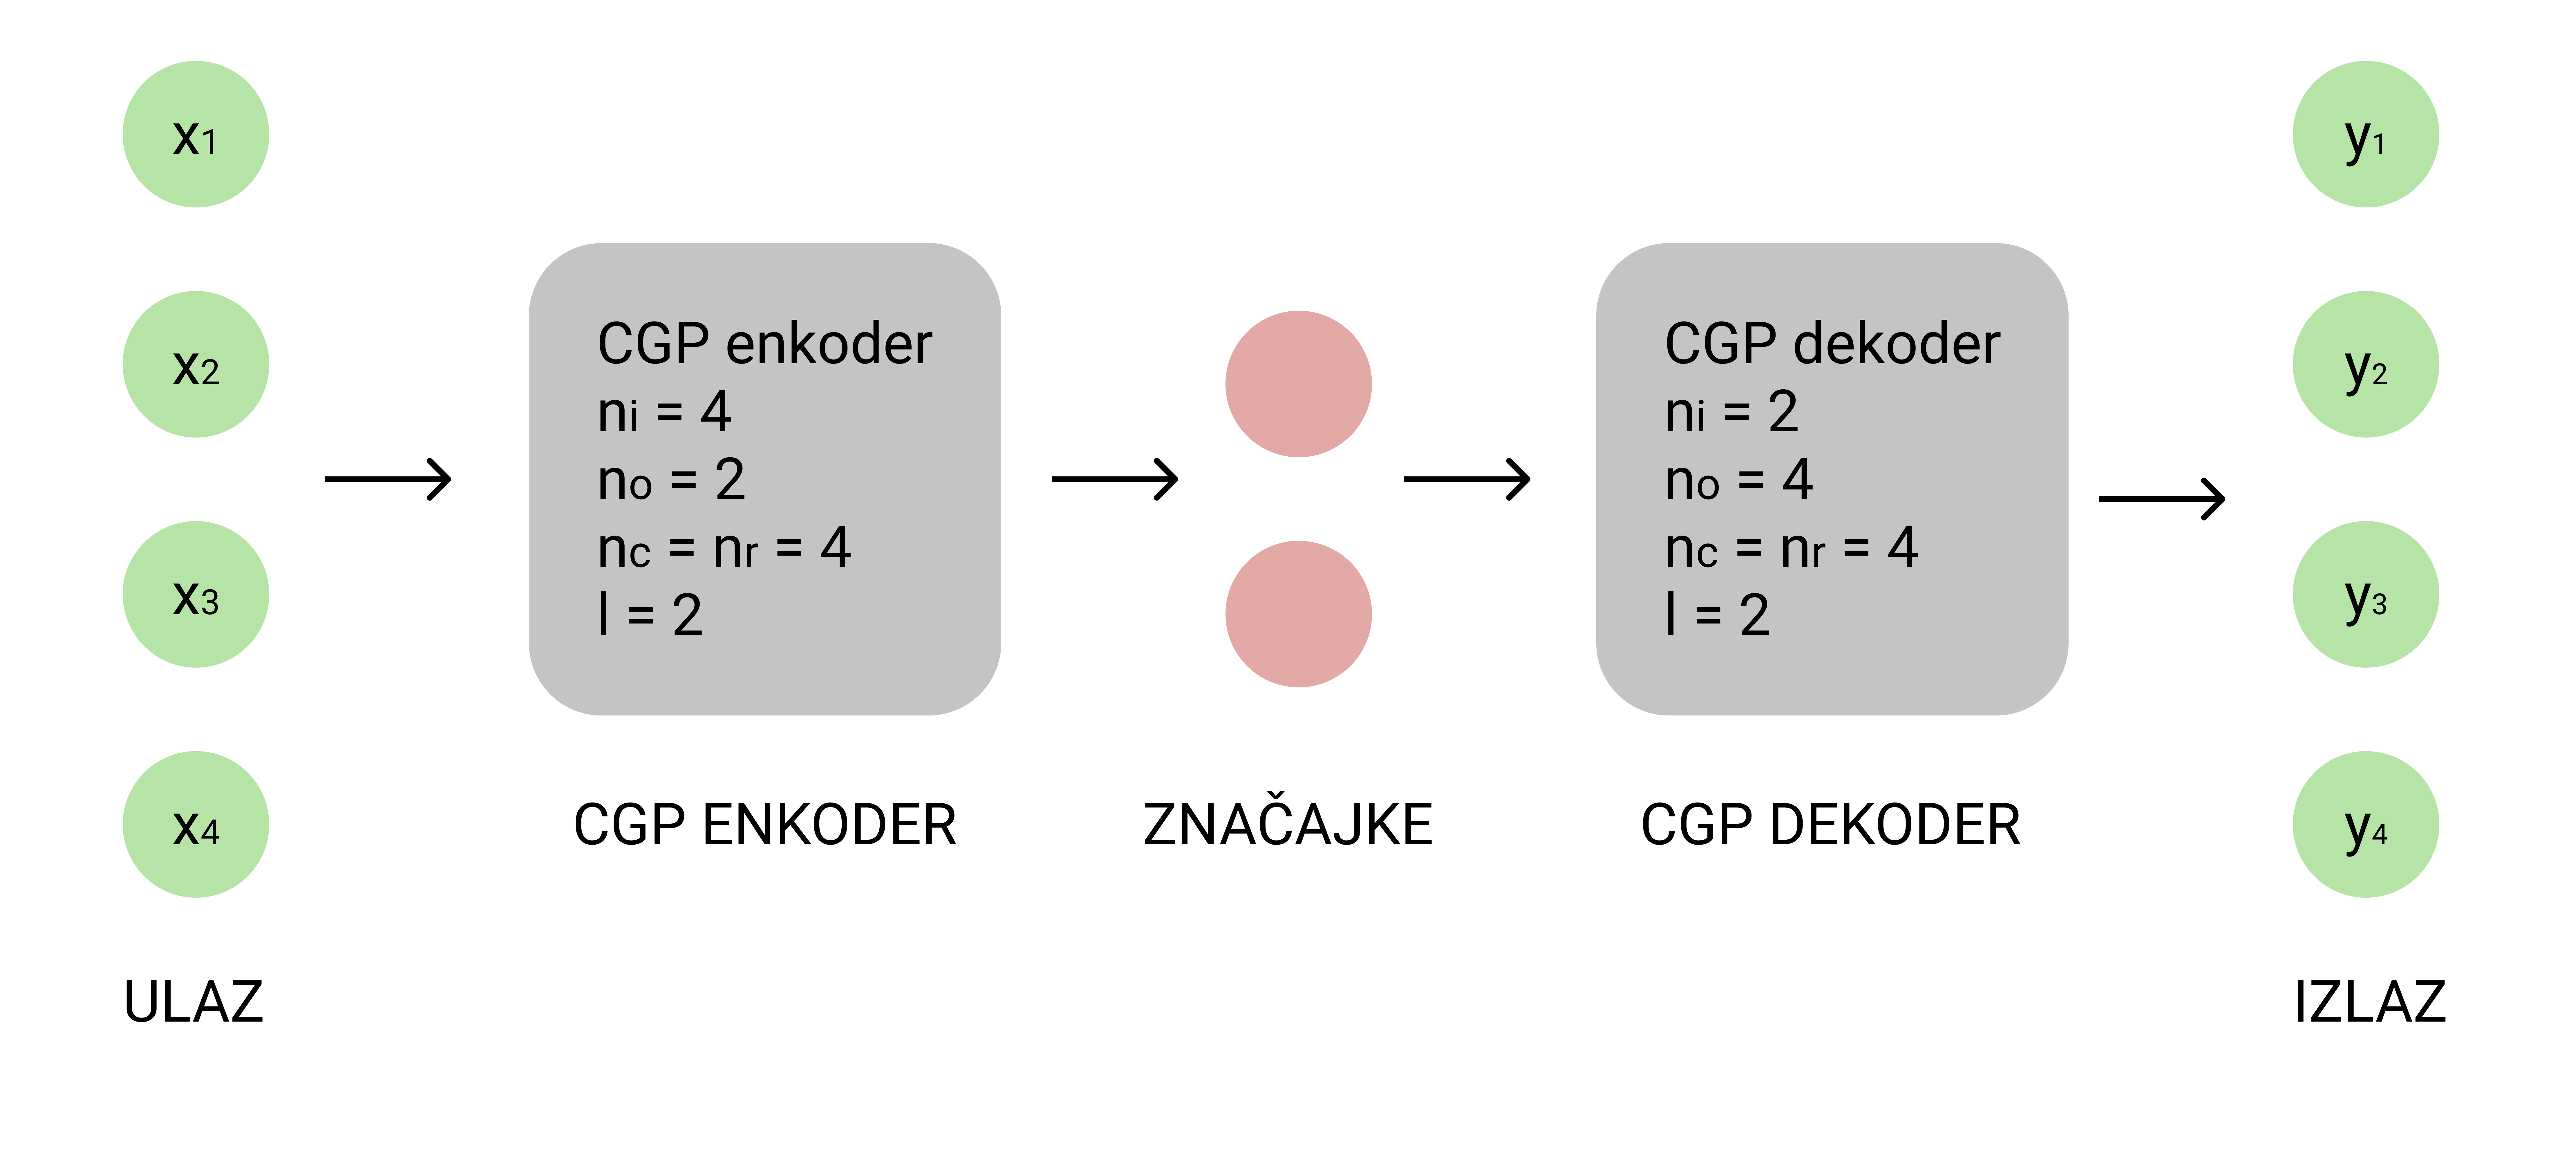
\includegraphics[width=\linewidth]{Illustrations/cgp_encoder_example.png}
	\caption{Prikaz predložene arhitekture \emph{CGPAE}. Korištenje dva neovisna CGP elementa u seriji. Izlazi enkodera odgovaraju značajkama. Ulaz dekodera odgovara broju značajki a izlaz ulazu u enkoder. Preciznije, izlaz enkodera je ulaz u dekoder.}
\end{figure}

\subsubsection{Algoritam}
